%!TEX root = ../report.tex
\section{Pitchfork}

Next, we show how to detect the pitchfork, continue on a non-trivial branch, recover the other non-trivial branch and lastly find the exact location of the bifurcation point. When we speak about the {\em upper} and {\em lower} branch, we refer to the non-symmetric branches with largest and smallest $\psi_{max}$ as shown in the bifurcation diagram of Figure~\ref{fig:bifurcation_diagram}.

\subsection{Detection}
The cheapest way to continue on the upper branch of the pitchfork is to break the anti-symmetry of the PDE temporarily. This is carried out by adding a non-symmetric forcing term to the equation controlled by a new parameter {\tt asym}, continuing only a tad in the new parameter, subsequently continuing in $Re$ past the pitchfork bifurcation point, and lastly restoring symmetry by bringing {\tt asym} back to 0. To be more precise, we replace the wind stress forcing term $\tau_x$ by
\begin{equation}
    \tau_x := -\eta \left( \frac{1 - \mathtt{asym}}{2 \pi} \cos(2\pi y) + \frac{\mathtt{asym}}{\pi} \cos(\pi y) \right),
\end{equation}
such that the corresponding term in the right-hand side of the PDE~\eqref{eq:pde} becomes
\begin{equation}
    -\frac{\partial \tau_x}{\partial y} = -\eta ((1 - \mathtt{asym})\sin(2\pi y) + \mathtt{asym}\sin(\pi y)).
\end{equation}
This clearly breaks the anti-symmetry: $\partial_y \tau_x(y) \neq -\partial_y \tau_x(1 - y).$ We add the parameter $\mathtt{asym}$ at $Re = 16$ and continue in $\mathtt{asym}$ for two steps of $\Delta s = 0.1.$ We then continue in $Re$ until $Re \approx 31.$ At this point it becomes clear we have passed the pitchfork bifurcation point, by judging the behaviour of the solution as shown in Figure~\ref{fig:pitch_detection}. If we look at $\psi_{max}$ as a function of $Re,$ we see interesting behaviour around $Re \approx 29,$ where it suddenly increases and then flattens. Also the effective step size in $Re$ decreases while $\Delta s$ is kept constant at $0.1$; this could mean that the solution changes more rapidly. Even more pronounced is the graph of $\psi_{max} + \psi_{min}$ where we not only see the small disturbance in symmetry around $Re = 16,$ but as well how it blows up past $Re = 29.$ Another way to detect the bifurcation point is to look at a specific point of the solution such as $\psi(\tfrac{1}{8}, \tfrac{1}{8})$ or $\psi(\tfrac{3}{8}, \tfrac{3}{8})$ where a qualitative change in behaviour appears after $Re = 29.$

At $Re \approx 31$, we bring back $\texttt{asym}$ to $0.$ Next we continue to $Re = 40$ at which point we obtain the solution as plotted in Figure~\ref{fig:question_e}. Now that we are on a branch of non-symmetric steady states, we can easily get on its anti-symmetric counterpart (the lower branch) by continuing backwards in $Re$ from $Re = 40$ to $Re_p$ and then all the way to $Re = 40$ again. This is done by setting $\Delta s = -1.$ We plot the solution in Figure~\ref{fig:question_e_lower}. Although it is not immediately clear from the plot, we verified in Matlab the lower branch is indeed anti-symmetric around $y = 0.5$ compared with the upper branch.

\begin{figure}[p]
    \centering
    \label{fig:pitch_detection}
    \centerline{\includegraphics[width=1.3\textwidth]{images/pitch_detection.pdf}}
    \caption{Detection of the pitchfork.}
\end{figure}

\begin{figure}[p]
    \centering
    \centerline{
    \begin{subfigure}[b]{0.6\textwidth}
        \includegraphics[width=\textwidth]{images/e_psi.eps}
        \caption{Streamfunction $\psi$ at $Re = 40$.}
        \label{fig:question_e_psi}
    \end{subfigure}
    ~
    \begin{subfigure}[b]{0.6\textwidth}
        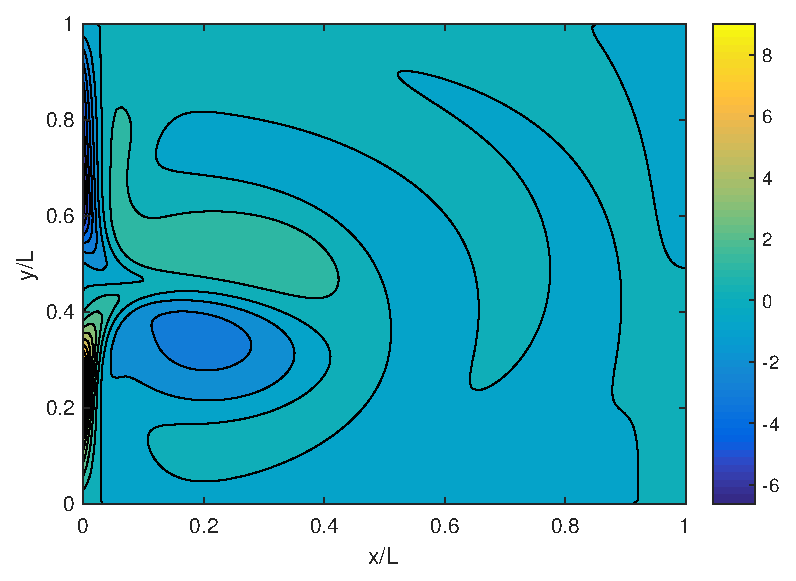
\includegraphics[width=\textwidth]{images/e_zeta.eps}
        \caption{$\zeta$ at $Re = 40$.}
        \label{fig:question_e_zeta}
    \end{subfigure}
    }
    \caption{Solutions on the upper branch of the pitchfork.}\label{fig:question_e}
\end{figure}


\begin{figure}[p]
    \centering
    \centerline{
    \begin{subfigure}[b]{0.6\textwidth}
        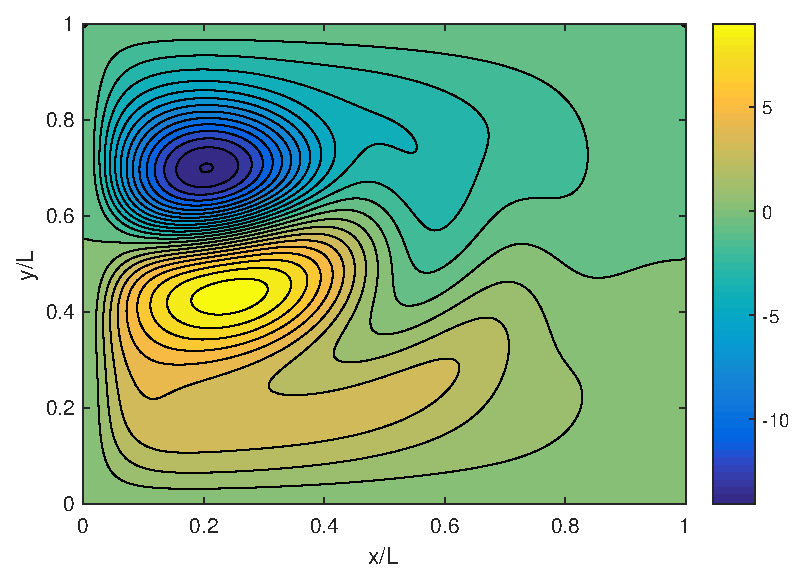
\includegraphics[width=\textwidth]{images/e_psi_lower.eps}
        \caption{Streamfunction $\psi$ at $Re = 40$.}
        \label{fig:question_e_psi_lower}
    \end{subfigure}
    ~
    \begin{subfigure}[b]{0.6\textwidth}
        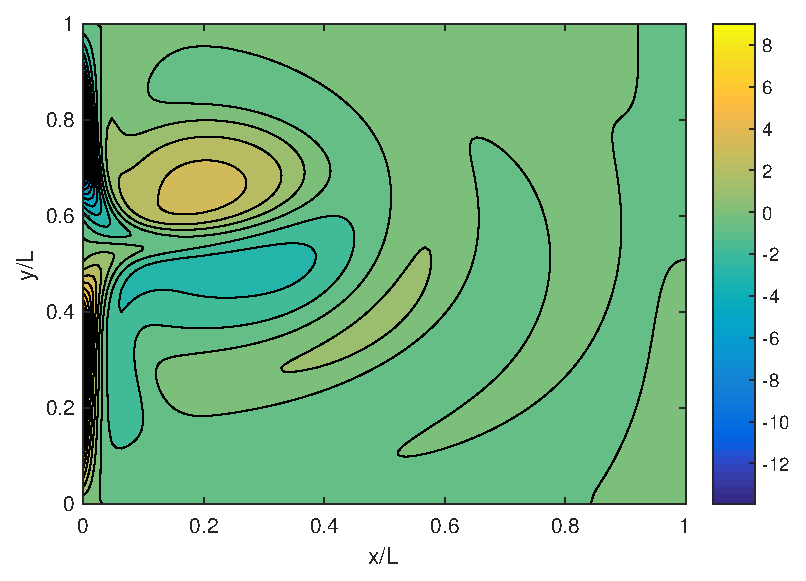
\includegraphics[width=\textwidth]{images/e_zeta_lower.eps}
        \caption{$\zeta$ at $Re = 40$.}
        \label{fig:question_e_zeta_lower}
    \end{subfigure}
    }
    \caption{Solutions on the lower branch of the pitchfork.}\label{fig:question_e_lower}
\end{figure}

\begin{figure}[p]
    \includegraphics[width=\textwidth]{images/eigenvalues.pdf}
    \caption{An eigenvalue becomes positive after increasing the Reynolds number slightly.}
    \label{fig:eigenvaluespitch}
\end{figure}

\newpage

\subsection{Finding its location and type}
In dynamical systems, the most fruitful way to assess non-linear systems is to look at their linearized approximation around an equilibrium. Via the Hartman-Grobman theorem the behaviour of the linearized system is under very mild conditions locally topologically equivalent to the non-linear system. Since we are always moving over an equilibrium, we can inspect the linearization $\*{\tilde u}$ of~\eqref{eq:ode} which is simply

\begin{equation}
    M\frac{d \*{\tilde u} }{d t} := DF_{\*u}\*{\tilde{u}}.
\end{equation}
To find the exact location of the pitchfork bifurcation and to inspect stability of the system, we can hence look at the generalized eigenvalue problem
\begin{equation}\label{eq:eigs}
    DF_{\*u}(\*u^*)x = \lambda M x,
\end{equation}
where $\*u^*$ is a given equilibrium of the ODE~\eqref{eq:ode}.

To solve the generalized eigenvalue problem~\eqref{eq:eigs}, we use an eigenvalue solver (JDQZ) with a real target $\tau$ near the origin. This way we can detect a change of sign in the eigenvalues, and use the secant process to find exactly at which Reynolds number the pitchfork occurs. In Figure~\ref{fig:eigenvaluespitch} we show how the eigenvalue closest to the origin moves past the imaginary axis. It turns out that the ``exact'' location of the pitchfork is at $Re_p \approx 29.5112$.

Lastly, we use the eigenvalue solver to compute some eigenvalues on all branches away from the pitchfork and check the sign of the real part. It turns out that the pitchfork consists of three stable parts and one non-stable part, which fits in the category of {\em supercritical} pitchforks. 


